

\documentclass[a4paper,UKenglish,cleveref, autoref, thm-restate]{lipics-v2021}

\bibliographystyle{plainnat}
% \bibliographystyle{plainurl}% the mandatory bibstyle
\usepackage{comment}
\usepackage{todonotes}
\usepackage{amsthm}
\usepackage{amsmath} 
\usepackage{amsfonts}
\usepackage{natbib}
\usepackage{algorithm}
\usepackage{algorithmicx}
\usepackage{algpseudocode}
\usepackage{booktabs}
\usepackage{graphicx}   % For including graphics
\usepackage{pgf}        % Allows PGF figures
\usepackage{caption}  


%\newtheorem{theorem}{Theorem}
%\newtheorem{problem}{Problem}
%\newtheorem{definition}[theorem]{Definition}


\title{Learning Neural Networks Using Mixed Integer Programming}

%\titlerunning{Dummy short title} %TODO optional, please use if title is longer than one line



\author{Viljar Helgestad Gjerde}{Department of Informatics, University of Bergen, Norway}{viljar.gjerde@student.uib.no}{ORCID HERE}{}


\author{Mateus de Oliveira Oliveira}{Department of Computer and System Sciences, Stockholm University, Sweden \and Department of Informatics, University of Bergen, Norway}{oliveira@dsv.su.se}{https://orcid.org/0000-0001-7798-7446}{}


\author{Wim Van den Broeck}{Department of Informatics, University of Bergen, Norway}{wim.broeck@uib.no}{ORCID HERE}{}


\authorrunning{V. Helgestad Gjerde and M. de Oliveira Oliveira and W. Van den Broeck} %TODO mandatory. First: Use abbreviated first/middle names. Second (only in severe cases): Use first author plus 'et al.'

\Copyright{Viljar Helgestad Gjerde and Mateus de Oliveira Oliveira and Wim Van den Broeck} %TODO mandatory, please use full first names. LIPIcs license is "CC-BY";  http://creativecommons.org/licenses/by/3.0/

\ccsdesc[500]{Computing methodologies~Machine learning}
\ccsdesc[500]{Theory of computation~Integer programming}

\keywords{Mixed Integer Programming, Neural Networks} %TODO mandatory; please add comma-separated list of keywords

\category{} %optional, e.g. invited paper

\relatedversion{} %optional, e.g. full version hosted on arXiv, HAL, or other respository/website
%\relatedversiondetails[linktext={opt. text shown instead of the URL}, cite=DBLP:books/mk/GrayR93]{Classification (e.g. Full Version, Extended Version, Previous Version}{URL to related version} %linktext and cite are optional

%\supplement{}%optional, e.g. related research data, source code, ... hosted on a repository like zenodo, figshare, GitHub, ...
%\supplementdetails[linktext={opt. text shown instead of the URL}, cite=DBLP:books/mk/GrayR93, subcategory={Description, Subcategory}, swhid={Software Heritage Identifier}]{General Classification (e.g. Software, Dataset, Model, ...)}{URL to related version} %linktext, cite, and subcategory are optional

\funding{Research Council of Norway, project numbers 288761 and 326537.}%optional, to capture a funding statement, which applies to all authors. Please enter author specific funding statements as fifth argument of the \author macro.

%\acknowledgements{I want to thank \dots}%optional

%\nolinenumbers %uncomment to disable line numbering



%Editor-only macros:: begin (do not touch as author)%%%%%%%%%%%%%%%%%%%%%%%%%%%%%%%%%%
\EventEditors{John Q. Open and Joan R. Access}
\EventNoEds{2}
\EventLongTitle{42nd Conference on Very Important Topics (CVIT 2016)}
\EventShortTitle{CVIT 2016}
\EventAcronym{CVIT}
\EventYear{2016}
\EventDate{December 24--27, 2016}
\EventLocation{Little Whinging, United Kingdom}
\EventLogo{}
\SeriesVolume{42}
\ArticleNo{23}
%%%%%%%%%%%%%%%%%%%%%%%%%%%%%%%%%%%%%%%%%%%%%%%%%%%%%%

\begin{document}



\maketitle



\section{Introduction}



\section{A distribution that is hard for standard graph neural networks.}





\section{Preliminaries}

\section{Graph Theoretical Foundations}

In this section, we establish the fundamental definitions that will be used throughout this paper.

\subsection{Undirected Graph}
An \textit{undirected graph} is defined as a pair $G = (V, E)$, where:
\begin{itemize}
    \item $V$ is a finite set of vertices (or nodes).
    \item $E \subseteq \{ \{u,v\} \mid u,v \in V, u \neq v\}$ is a set of edges, where each edge is an unordered pair of distinct vertices.
\end{itemize}
Since the graph is undirected, if $\{u,v\} \in E$, then there exists a connection between $u$ and $v$, and the relationship is bidirectional.

A useful way to represent $G$ is through its \emph{adjacency matrix} $\mathbf{A} \in \{0,1\}^{n \times n}$, where $n = |V|$ is the number of nodes. The adjacency matrix is defined as:

\begin{equation}
A_{ij} =
\begin{cases}
    1, & \text{if } \{i,j\} \in E, \\
    0, & \text{otherwise}.
\end{cases}
\end{equation}

Since the graph is undirected, $\mathbf{A}$ is symmetric, meaning that $A_{ij} = A_{ji}$ for all $i,j \in V$. The diagonal entries $A_{ii}$ are typically zero unless self-loops are explicitly included in the graph. This matrix representation provides a convenient way to encode the graph structure for computational methods, including graph neural networks.

\subsection{Clique}

A \textit{clique} in a graph $G = (V, E)$ is a subset of vertices $C \subseteq V$ such that every pair of vertices in $C$ is adjacent, meaning that for all $u, v \in C$ with $u \neq v$, the edge $\{u,v\}$ is present in $E$. 

A \textit{clique} in a graph $G = (V, E)$ is a subset of vertices $C \subseteq V$ such that every pair of vertices in $C$ is adjacent, meaning that for all $u, v \in C$ with $u \neq v$, the edge $\{u,v\}$ is present in $E$. 

The \textit{k-clique problem}, which asks whether a graph contains a clique of size $k$, is NP-complete when $k$ is part of the input \citep{karp1972reducibility}, but for a fixed constant $k$, it can be solved in polynomial time by enumerating all $\binom{|V|}{k}$ possible subsets of vertices and checking for completeness. More specifically, \citet{vassilevska2009efficient} show that the problem can be solved in $O\left(\frac{n^k}{(\varepsilon \log n)^{k-1}}\right)$ time and $O(n^\varepsilon)$ space for all $\varepsilon > 0$, achieving an improvement over the naive $O(n^k)$ approach.


\subsection{Graph Coloring}
A \textit{proper coloring} of a graph $G = (V, E)$ is an assignment of colors to vertices such that no two adjacent vertices share the same color. Formally, a function $f: V \to \{1,2,\dots,r\}$ is an $r$-coloring if for every edge $\{u,v\} \in E$, it holds that $f(u) \neq f(v)$. The \textit{chromatic number} $\chi(G)$ is the smallest integer $r$ for which an $r$-coloring exists.

The problem of determining whether a graph can be colored with at most $r$ colors, known as the \textit{graph coloring problem}, is NP-complete for general graphs when $r \geq 3$ \citep{karp1972reducibility}. However, for fixed values of $r$, specialized algorithms can solve the problem more efficiently. In particular, the $3$-coloring problem can be solved in $O(1.3289^n)$ time using an improved branching algorithm \citep{beigel2000finding}. 

\subsection{\textit{k}-Clique vs \textit{r}-Coloring Problem}




The \textit{$k$-clique vs. $r$-coloring problem} is a classification problem. Given integers $k$ and $r$, with $r < k$, and a graph $G$ that is promised to either contain a $k$-clique or be $r$-colorable, the task is to determine which is the case. While both the $k$-clique and $r$-colorability problems are individually NP-complete, this specific problem is not classified as NP-complete since the input graph satisfies exactly one of the two mutually exclusive properties.

This problem can be solved efficiently in certain graph classes, such as perfect graphs and their generalizations. In perfect graphs, the chromatic number equals the size of the largest clique, simplifying the determination of $r$-colorability and the presence of $k$-cliques. \todo{elaborate on why this helps, and why k and r can be calculated in polynomial time} For general graphs, an efficient approach relies on the Lovász theta function, $\vartheta(G)$. The Lovász Sandwich Theorem establishes the bounds:
\begin{equation}
    \alpha(G) \leq \vartheta(G) \leq \bar{\chi}(G),
\end{equation}
\citep{lovasztheta}
where $\alpha(G)$ is the independence number, representing the size of the largest independent set in $G$, and $\bar{\chi}(G)$ is the fractional chromatic number, a relaxation of the chromatic number that allows fractional color assignments. While computing $\alpha(G)$ and $\bar{\chi}(G)$ is NP-hard, the Lovász theta function is efficiently computable via semidefinite programming (SDP), making it an efficient way of separating the two classes. 


% \begin{enumerate}
%     \item The graph $G$ contains a clique of size at least $k$, i.e., there exists a subset $C \subseteq V$ with $|C| \geq k$ such that every pair of vertices in $C$ is connected.
%     \item The graph $G$ can be colored using at most $r$ colors, i.e., there exists a valid $r$-coloring function $f: V \to \{1,2,\dots,r\}$.
% \end{enumerate}

% This problem is significant in theoretical computer science and combinatorial optimization, as it relates to NP-hard problems such as \textsc{Clique} and \textsc{Graph Coloring}. The interplay between maximum clique size and chromatic number has implications in graph theory, information theory, and constraint satisfaction problems.



\subsection{Graph Convolutional Networks}
\label{sec:GCN}

To distinguish r-colorable graphs from graphs with k-cliques, we adopt the
\textbf{Graph Convolutional Network (GCN)} model proposed by \citet{GCNKipf2016} as the
core model in our pipeline.

\paragraph{Local Graph Convolutions.}  
Each node $i$ in the graph is represented with an \emph{embedding}, a vector in $\mathbb{R}^{d_{\ell}}$, where $ d_{\ell} $ is the dimensionality of the embedding at layer $ \ell $, commonly described as the number of channels. Initially ($\ell = 0$), this embedding is simply the node’s feature vector. These features can be combined into the matrix $\mathbf{H}^{(\ell)} \in \mathbb{R}^{n \times d_{\ell}}$, where each row corresponds to the embedding of a node.  

A \emph{Graph Convolutional Network (GCN) layer} updates node embeddings by aggregating information from neighboring nodes through applying a learned transformation. This transformation is parameterized by a trainable weight matrix $ \mathbf{W}^{(\ell)} \in \mathbb{R}^{d_{\ell} \times d_{\ell + 1}} $, which maps embeddings from dimension $ d_{\ell} $ to a new dimension $ d_{\ell+1} $ at the next layer. The node embeddings are updated as follows:

\begin{equation}   
    \mathbf{H}^{(\ell+1)} 
    = \sigma\!\Big(
        \widetilde{\mathbf{D}}^{-\frac12} \,
        \widetilde{\mathbf{A}} \,
        \widetilde{\mathbf{D}}^{-\frac12} \,
        \mathbf{H}^{(\ell)} \,
        \mathbf{W}^{(\ell)}
    \Big),
\end{equation}

where $ \tilde{\mathbf{A}} = \mathbf{A} + \mathbf{I} $ is the adjacency matrix with added self-loops to ensure that each node retains information from its own embedding. $ \tilde{\mathbf{D}}_{ii} = \sum_j \tilde{\mathbf{A}}_{ij} $ is a diagonal degree matrix that normalizes the adjacency matrix. Lastly, $ \sigma(\cdot) $ is a nonlinear activation function such as ReLU or sigmoid, which is crucial for enabling the model to learn complex, non-linear relationships—without it, the layer would merely perform a linear transformation, limiting the network’s expressive power.  

Stacking multiple GCN layers allows each node embedding to incorporate information from progressively larger neighborhoods. This is because each layer aggregates features from a node’s immediate neighbors. With each additional layer, a node’s representation is updated based on its direct neighbors, which themselves have already integrated information from their own neighbors in the previous layer. Consequently, deeper GCNs enable nodes to capture higher-order structural and semantic information across the graph.

% \paragraph{Local Graph Convolutions.}
% Each node $i$ in the graph is represented with an \emph{embedding}, a vector in $\mathbb{R}^{d_{\ell}}$. Initially, this embedding is simply the node features. These features can be combined into the matrix $\mathbf{H}^{(\ell)} \in \mathbb{R}^{n \times d_{\ell}}$, where each row corresponds to the embedding of a node.

% A \emph{Graph Convolutional Network (GCN) layer} is a transformation that updates node embeddings, by aggregating information from neighboring nodes. A GCN layer is defined by its trainable weight matrix $\mathbf{W} \in \mathbb{R}^{d_\ell \times d_{\ell + 1} }$. The node embeddings in a graph are then updated as follows:

% \begin{equation}   
%     \mathbf{H}^{(\ell+1)} 
%     = \sigma\!\Big(
%         \widetilde{\mathbf{D}}^{-\frac12} \,
%         \widetilde{\mathbf{A}} \,
%         \widetilde{\mathbf{D}}^{-\frac12} \,
%         \mathbf{H}^{(\ell)} \,
%         \mathbf{W}^{(\ell)}
%     \Big),
% \
% \end{equation}

% where $\tilde{A} = A + \mathbb{I}$ is the adjacency matrix $A$ of the node, with the identity matrix representing self-loops added to ensure the node's own embeddings are preserved. $\tilde{D}_{ii} = \Sigma_j \tilde{A}_{ij}$ is a diagonal matrix representing the degree of node $i$. Lastly, $\sigma(\cdot)$ is a nonlinear function such as the sigmoid or ReLU function, without which, the layer would just be a linear transformation unable to represent non-linear and thus arbitrary functions.  Stacking multiple GCN layers allows each node embedding to incorporate information from progressively larger neighborhoods. This is because each layer aggregates features from a node’s immediate neighbors. With each additional layer, a node’s representation is updated based on its direct neighbors, which themselves have already integrated information from their own neighbors in the previous layer. 

\paragraph{Graph-Level Classification.}
While GCNs were originally popularized for node-level classification tasks, our objective is
to classify entire graphs according to whether it is $r$-colorable or contains an $k$-clique. To adapt the GCN to graph-level classification, we apply global averaging across all nodes after the final GCN layer.
\begin{equation}
   \mathbf{z} 
   = \mathrm{mean}\bigl(\mathbf{H}^{(L)}\bigr) \quad \in \mathbb{R}^{d_L}
\end{equation}
where $\mathbf{H}^{(L)} \in \mathbb{R}^{N \times d_{L}}$ is the final layer output, and
$\mathrm{mean}(\cdot)$ aggregates node embeddings into a single graph-level representation $\mathbf{z}$. We then feed $\mathbf{z}$ into one or more fully connected layer(s), ending in a single output neuron used for classification. We detail the full architecture and hyperparameters in \cref{sec:experiments}.
\todo{Fix reference when this section is written}

\paragraph{Tok-k pooling}

In graph neural networks, pooling methods help reduce the size of a graph while preserving critical structural and feature-based information, making them particularly useful for tasks that depend on specific substructures. Top-K Pooling, as developed and discussed by \citet{topk1,topk2,topk3}, selectively retains the most informative nodes based on learnable importance scores. This allows the model to focus on regions of the graph that are most relevant to a given classification task. When determining whether a graph is $r$-colorable or contains a $k$-clique, certain nodes and their connections are far more influential than others. By using Top-K Pooling, the model can prioritize these key regions, reducing irrelevant complexity while retaining the features necessary to distinguish between different graph classes. The top-k algorithm is shown in \cref{alg:topk}, where $\odot$ is elementwise multiplication.

\begin{algorithm}
\caption{Top-K Pooling Algorithm}
\label{alg:topk}
\begin{algorithmic}[1]
    \State \textbf{Input:} Node feature matrix $\mathbf{X} \in \mathbb{R}^{N \times d}$, adjacency matrix $\mathbf{A} \in \mathbb{R}^{N \times N}$, learnable projection vector $\mathbf{p} \in \mathbb{R}^{d}$, pooling ratio $k$
    \State \textbf{Output:} Pooled node features $\mathbf{X'}$, pooled adjacency matrix $\mathbf{A'}$
    \vspace{0.2cm}
    
    \State \textbf{Compute node importance scores:}
    \[
    \mathbf{y} = \frac{\mathbf{X} \mathbf{p}}{\|\mathbf{p}\|}
    \]
    
    \State \textbf{Select top-k nodes based on scores:}
    \[
    \mathbf{i} = \text{top-k}(\mathbf{y}, k)
    \]
    
    \State \textbf{Update node features:}
    \[
    \mathbf{X'} = (\mathbf{X} \odot \tanh(\mathbf{y}))_{\mathbf{i}}
    \]
    
    \State \textbf{Update adjacency matrix:}
    \[
    \mathbf{A'} = \mathbf{A}_{\mathbf{i}, \mathbf{i}}
    \]

    \State \textbf{Return} $\mathbf{X'}$, $\mathbf{A'}$
\end{algorithmic}
\end{algorithm}

% Formally, top-k takes a graph defined by the feature-matrix $\mathbf{X}$ and the adjacency matrix $\mathbf{A}$, and calculates the pooled versions $\mathbf{X'}$ and $\mathbf{A'}$ as shown in 

\paragraph{Model rationale}
\todo{Rewrite and reposition}
We posit that a Graph Convolutional Network (GCN) is particularly suitable for separating r-colorable graphs from k-clique graphs due to its ability to effectively process both node features and the structural relationships defined by adjacency. GCNs should be able to capture the high-degree patterns of cliques and distinguish these from r-colorable configurations by aggregating degree information in the context of each node’s neighbors. They also excel at handling irregular graph structures, making them versatile for graphs of varying sizes.

% \paragraph{Model rationale}
% From a purely combinatorial perspective, detecting large cliques or verifying whether a graph is r-colorable presents significant challenges (see Section~\ref{sec:cliques_coloring}). Our hypothesis posits that Graph Convolutional Networks (GCNs) naturally leverage local structures—dense subgraph patterns indicative of cliques and neighborhood sparsity. By propagating features through the graph, GCNs effectively integrate multi-hop connectivity, which may correlate with specific structural patterns. Consequently, when trained on examples that are either r-colorable or contain k-cliques (or labeled with a more detailed classification scheme), the network can learn representations that distinguish between these two cases.


\section{Graph generation}

% In this section we describe how we generate random graphs that either belong to the r-colorable group or the k-clique group. For the r-colorable graphs, the nodes are first randomly given a color, and then edges are randomly assigned with probability \deprob for each pair of nodes with different colors. For the k-clique graphs, $k$ nodes are first chosen to be part of a clique, and fully connected before edges are added randomly with \deprob for all possible pairs of nodes. Each node in a GNN is associated with one or more features. For our experiments, we use the degree of the node as its feature. \Cref{alg:r-colorable,alg:k-clique} describe the graph generation algorithms in more detail.

In this section, we outline the process for generating random graphs belonging to either the $r$-colorable group or the $k$-clique group. For $r$-colorable graphs, each node is randomly assigned a color, and edges are added between nodes of different colors with a probability of $p$. For $k$-clique graphs, $k$ nodes are first selected to form a fully connected clique, after which additional edges are randomly added between all node pairs with probability $q$. In a GNN, each node is associated with one or more features; in our experiments, we use node degree as the sole feature. \Cref{alg:r-colorable,alg:k-clique} provide a detailed description of the graph generation algorithms.


\begin{algorithm}
\caption{Generating a Graph with an $k$-Clique}
\label{alg:k-clique}
\begin{algorithmic}[1]
    \Require 
        \begin{itemize}
            \item $N$: Total number of nodes in the graph
            \item $k$: Size of the clique
            \item $p$: Probability of adding edges outside the clique.
        \end{itemize}
    \Ensure A graph with a fully connected $k$-clique and additional edges based on $p$.

    \State \textbf{Select Nodes for the Clique:}
        \begin{itemize}
            \item Randomly choose $k$ nodes from the total $N$ to form the clique.
        \end{itemize}
    
    \State \textbf{Create Clique Edges:}
        \begin{itemize}
            \item For every pair of nodes in the clique, add an edge between them.
        \end{itemize}

    \State \textbf{Create Edges for Other Nodes:}
        \begin{itemize}
            \item For all pairs of nodes that are not both in the clique:
            \begin{itemize}
                \item Add an edge with probability $p$ between those nodes.
            \end{itemize}
        \end{itemize}

    \State \textbf{Combine Edges:}
        \begin{itemize}
            \item Merge the edges from the clique with the edges between other nodes.
        \end{itemize}

    \State \textbf{Generate Node Features:}
        \begin{itemize}
            \item For each node, compute its degree. Use this as the node's feature.
        \end{itemize}

   \State \textbf{Output: Adjacency Matrix, Node Features}
        \begin{itemize}
            \item Construct an adjacency matrix $\mathbf{A}$ from the list of edges.
            \item Create a feature matrix $\mathbf{X}$, where each row represents a node's feature.
        \end{itemize}


\end{algorithmic}
\end{algorithm}


\begin{algorithm}
\caption{Generating a $r$-Colorable Graph}
\label{alg:r-colorable}
\begin{algorithmic}[1]
    \Require 
        \begin{itemize}
            \item $N$: Total number of nodes in the graph
            \item $r$: Number of colors (used to group nodes into $r$ separate sets)
            \item $q$: Probability of adding edges between each pair of nodes of different colors
        \end{itemize}
    \Ensure A graph where nodes are grouped into $r$ colors, and edges exist only between nodes of different colors.

    \State \textbf{Assign Colors to Nodes:}
        \begin{itemize}
            \item Assign a random color (from $0$ to $r-1$) to each node.
        \end{itemize}

    \State \textbf{Add Edges Between Different Colors:}
        \begin{itemize}
            \item For every pair of nodes:
            \begin{itemize}
                \item Check if their colors are different.
                \item If they are, add an edge with probability $q$ between those nodes.
            \end{itemize}
        \end{itemize}

    \State \textbf{Generate Node Features:}
        \begin{itemize}
            \item For each node, compute its degree (number of edges). Use this as the node's feature.
        \end{itemize}

    \State \textbf{Output: Adjacency Matrix, Node Features}
        \begin{itemize}
            \item Construct an adjacency matrix $\mathbf{A}$ from the list of edges.
            \item Create a feature matrix $\mathbf{X}$, where each row represents a node's feature.
        \end{itemize}

\end{algorithmic}
\end{algorithm}



\section{Average Degree vs. Clique Coloring}
\subsection{Architecture (1-Filter GNN)}



\subsection{Clique versus coloring is easy on random graphs}

\begin{itemize}
\item Explain that it is a useful thing to have a network that solves combinatorail problems on random graphs because one usually cannot predcit the structure of hte graphs that are givesn as input. 
\item On random Erdos-Reny graphs the clicque coloroing principle is easy due to the fact that 
the average degree of a random graph with a k-clique is significnatly distinct from the average degree of a a random graph that is (k-1)-colorable: 
\item State the theorem: 1) Random graphs with a k-clique have average degree X
2)Random graphs that admit a k-1 coloring have average degree Z
\item Graph is equivalen to WL, and these can easily separate graphs with distinct average degrees. 
\item Put experiments showing this. 
\end{itemize}


\subsection{Average degree algorithm}
Due to the differences between \cref{alg:r-colorable} and \cref{alg:k-clique}, special care must be taken to avoid creating a trivial problem. Setting the $p = 0.5$ for both algorithms, will generate graphs with different average degrees ($d_{avg}$), as shown in \cref{fig:avg-degrees}. This gives rise to the following separation rule

\begin{equation}
\begin{cases}
r\text{-colorable}, & \text{if } d_{\text{avg}} < D \\
k\text{-clique}, & \text{otherwise}
\end{cases}
\end{equation}

where D is a threshold value for the network to learn. For the distributions shown in \cref{fig:avg-degrees}, any D between 36 and 46 will get 100\% accuracy. Indeed, even the simplest GCN, with a single layer and a single output feature, can quickly distinguish between the two classes.


\begin{figure}[htbp]
    \centering
    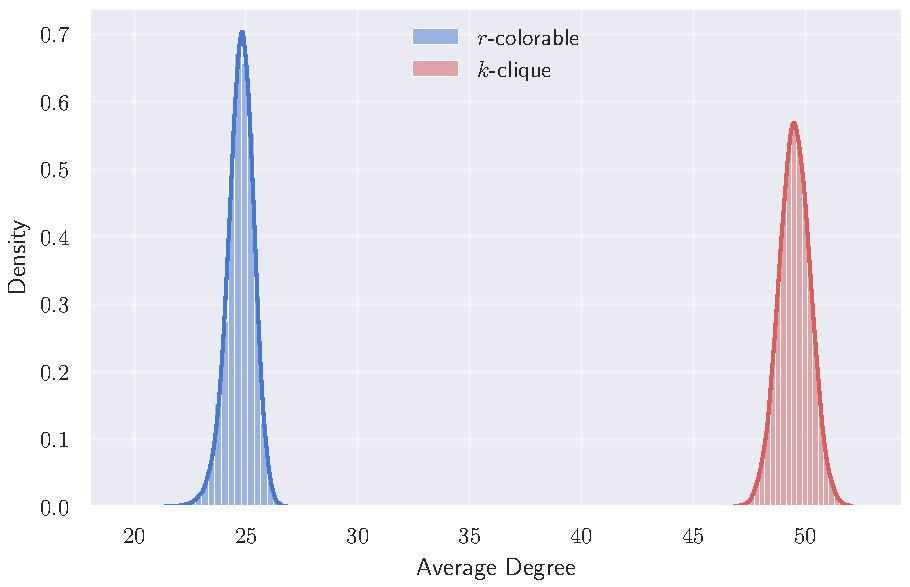
\includegraphics[width=0.9\linewidth]{plots/same-edgeprob.pdf}
    \caption{Histogram with KDE of average degrees for 2-colorable and 3-clique graphs with $N = 100$ and $p = 0.5$}
    \label{fig:avg-degrees}
\end{figure}

\subsection{Hard Cases for Average Degree}
\label{sec:hard-avg-degree}
To avoid the trivial case, we consider the case where the average degree for both graphs is equal. We achieve this by adjusting the edge probability when generating graphs. Starting with the expression for the expected average degree of a $r$-clique graph with $n$ nodes generated using \cref{alg:r-colorable}, we get

\renewcommand{\d}{d_{avg}}


\begin{equation}
\label{eq:r-edgeprob}
    \begin{split}
        \d = p(n-1)\frac{(r-1)}{r}
    \end{split}
\end{equation}
Similarly, for \cref{alg:r-colorable}, we get 
 

\begin{equation}
\label{eq:s-edgeprob}
    \begin{split}
        \d = \frac{s(s-1) + q(n-s) s  +2q (n -s) (n-s-1) }{n}
    \end{split}
\end{equation}
 Here the first term comes from edges within the clique, the second from edges between clique and non-clique nodes and the last from edges between non-clique nodes. Setting \cref{eq:s-edgeprob,eq:r-edgeprob} equal, we can solve for the $q$ where the expected average degree is the same.

\begin{equation}
    \begin{split}
        q = \frac{n  p \left(n - 1 \right)  \frac{r - 1}{r} - s \left(s - 1 \right)}{\left(n - s \right)  \left(n + s - 1 \right)}
    \end{split}
\end{equation}




The adjusted distributions are shown in \cref{fig:same-dist}. While the distribution of r-colorable graphs exhibits a slight left skew and has heavier tails, the high overlap coefficient of 0.9458 indicates that the two distributions are nearly identical. Empirical statistics based on 100,000 graphs with 100 nodes are presented in \cref{tab:same-dist}.


\begin{table}[htbp]
\caption{Empirical statistics based on 100,000 graphs with 100 nodes for the two distributions discussed in \cref{sec:hard-avg-degree}.}
\label{tab:same-dist}
\centering
\begin{tabular}{lrr}
\toprule
  Statistic & $r$-Colorable Graphs & $k$-Clique Graphs \\
\midrule
 Mean & 24.750 & 24.749 \\
 Variance & 0.370 & 0.370 \\
 Skewness & -0.511 & 0.022 \\
 Kurtosis & 1.186 & 0.005 \\
\midrule
  Overlapping Coefficient &\multicolumn{2}{r}{0.9458} \\
\bottomrule
\end{tabular}
\end{table}
% \begin{table}[htbp]
% \caption{Empirical statistics based on 100,000 graphs with 100 nodes for the two distributions discussed in \cref{sec:hard-avg-degree}.}
% \label{tab:same-dist}
% \centering
% \begin{tabular}{llrr}
% \toprule
%   Statistic & $r$-Colorable Graphs & $k$-Clique Graphs \\
% \midrule
%  Mean & 33.000 & 32.997 \\
%  Variance & 0.437 & 0.439 \\
%  Skewness & -0.236 & 0.008 \\
%  Kurtosis & 0.383 & -0.013 \\
% \midrule
%   Overlapping Coefficient (OVL) &\multicolumn{2}{r}{0.971} \\
% \bottomrule
% \end{tabular}
% \end{table}
\todo[color=green]{Include or remove histogram?}

\begin{figure}[htbp]
    \centering
    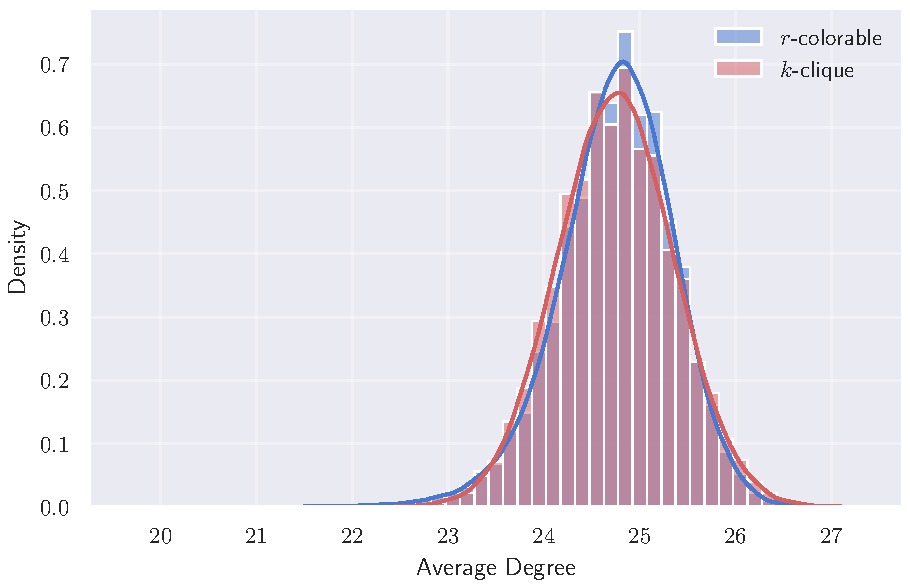
\includegraphics[width=0.9\linewidth]{plots/same-dist.pdf}
    \caption{Histogram with KDE of average degrees for 2-colorable and 3-clique graphs with $N = 100$ and edge probability adjusted to give the same average degree.}
    \label{fig:same-dist}
\end{figure}



\todo[inline]{I think that Vilijar also made some experiments stating that this distribution is easy for more general types of networks. }



\clearpage
\subsection{Architectures (GNNs + Linear Layers)}
\todo{Decide on which models to present and which results to present}
\todo[color=green]{Which r and s to present?}

\begin{figure}[ht]
    \centering
    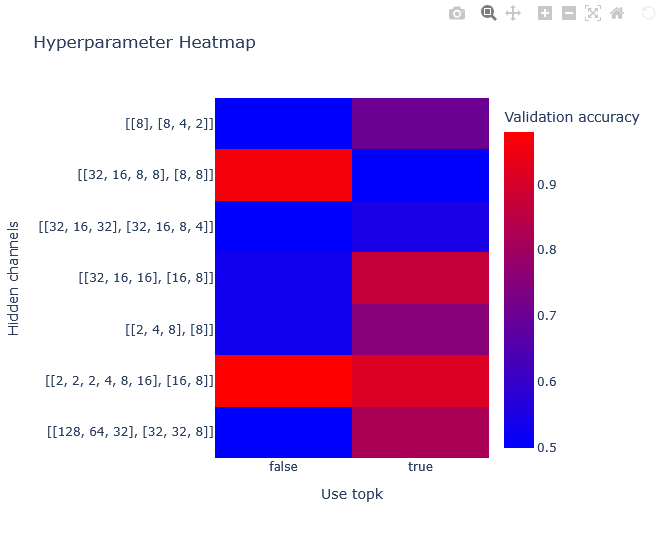
\includegraphics[width=0.8\linewidth]{plots/temp_results.png}
    \caption{Enter Caption}
    \label{fig:enter-label}
\end{figure}

\section{Improvements with the Top $k$ nodes technique}

\todo[inline]{Define pooling, and how it improves the process.}


\section{Connections with Weisfeiler Lehmant}
\begin{itemize}
\item paper about lower bounds for WL algorithm\url{https://people.cs.umass.edu/~immerman/pub/opt.pdf}
\item \url{https://arxiv.org/abs/1810.02244} 
\item Potentially hard case: A pair of graphs $G_1$ and $G_2$ that have the same 
WL-type, but one is $r$-colorable and the other has a $k$ clique. \todo{How to generate this?}
\end{itemize}

% \begin{abstract}
In this work, we investigate the use of mixed integer programming as a tool for learning neural networks with threshold gates. 
\end{abstract}

% \section{Introduction}
% \section{Preliminaries}


\begin{definition}[Dataset]
A $(n,k)$-dataset is a sequence $D = (D_0,D_1,...,D_{k-1})$ 
where each $D_i\subseteq \{0,1\}^n$ such that 
$D_i\cap D_j = \emptyset$ for each $i\neq j$.  
\end{definition}


\begin{problem}\label{Problem:MainProblem}
Given a Dataset $D$, learn a Network that is consistent with $D$. A relaxation of this problem consists in learning a network that is inconsistent with at most an $\varepsilon$ fraction of  the inputs. 
\end{problem}


\section{Networks with Threshold Gates and Integer Weights}

We will be operating with \textit{Threshold Gate Networks}. In this type of network, neurons are threshold gates. A gate with threshold $t$ fires if the sum of its inputs is at least $t$. In this first version, gates are assumed to be integers.  


\begin{problem}[Consistent Network]
\label{problem:Consistent}
Given an $(n,2)$-dataset $D = (D_0,D_1)$ and numbers 
$\delta$ (depth), $\omega$ (width), and $\tau$ (threshold), determine 
whether there exists a Threshold Gate Network $N$ 
such that $N$ rejects all strings in $D_0$ and accepts all 
strings in $D_1$. 
\end{problem}


\begin{problem}[Approximately Consistent Network]
\label{problem:Approximate}

Given an $(n,2)$-dataset $D = (D_0,D_1)$ and numbers 
$\delta$ (depth), $\omega$ (width), $\tau$ (threshold), and $\epsilon$, determine 
whether there exists a Threshold Gate Network $N$ 
such that $N$ rejects at least $(1-\epsilon)$ strings in $D_0$ and accepts at least $(1-\epsilon)$ strings in $D_1$. 
\end{problem}


\subsection{Evaluation of a network on a dataset}

\begin{itemize}
    \item Implement a program that reads a network (threshold circuit) from a file, and a dataset from another file and evaluates the circuit on each datapoint. 
\end{itemize}

% \section{Networks with Low Depth and High Width}


\section{Exact LP Formulation}

%TODO make notation as consistent with SAT as possible 


\subsection*{1) Parameters}
\begin{itemize}
    \item Dataset variables $x_{i,j}$: binary variable, 1 if and only if bit $j$ of string $i$ is equal to 1. 
    \item Dataset variables $t_{i}$: binary variable, 0 if string i belongs to class 0.
    \item depth $d$: Number of layers. 
    \item layer widths $w_l,  \forall l \in [\delta]$: Width of layer $l$. First width is equal to the input width. The last width is the output width.
\end{itemize}

\subsection*{2) Decision Variables}
\begin{itemize}
   \item  Threshold $g_{l,j}: \in \mathbb{N} \ |\  \mathbb{R}$ Decision variable for the threshold of each node $j$ at layer $l$. \\
   \item  weights $e_{l,j,j'}: \in \mathbb{N} \ |\  \mathbb{R}$  Decision variable for the weight of the edge from node $j$ in layer $l$ to node $j'$ in layer  $l+1$. \\ 
\end{itemize}

\subsection*{3) Auxiliary Variables}
\begin{itemize}
    \item Threshold reached $c_{l,j,i}$: Binary variable indicating whether node $j$ at layer $l$ fires for string $i$. \\ 
    \item wrong $m_i$: Binary variable indicating whether the prediction for string $i$ is wrong.
\end{itemize}




\subsection*{4) Constraints}
In the following constraints, M represents the upper bound of the left hand side. %TODO write explanation of each constraint
\begin{align*}
    &\sum_{j \in w_l} \left(\text{c}_{l,j,i} \times \text{e}_{l,j,j'}\right) - \text{g}_{l+1,j'} \leq M \times \text{c}_{l+1,j',i}, \quad \forall j' \in w_{l+1}, \forall i \in N, \\
    %
    &\sum_{j \in w_l} \left(\text{c}_{l,j,i} \times \text{e}_{l,j,j'}) - \text{g}_{l+1,j'} \geq 1 - M \times (1 - \text{c}_{l+1,j',i}\right), \quad \forall j' \in W, \forall i \in N, \\
    %
    &\text{c}_{1,j,i} = \text{x}_{i,j}, \quad \forall j \in w_1, \forall i \in N, \\
    %
    &\text{m}_i \geq \text{c}_{d,j',i} - \text{t}_i, \quad \forall i \in N, \\
    %
    &\text{m}_i \geq \text{t}_i - \text{c}_{d,j',i}, \quad \forall i \in N, \\
    %
    &\sum_{i \in N} m_i \leq \epsilon.
\end{align*}

By setting $\epsilon = 0$ the exact formulation is achieved. 


\subsection*{5) Objective Function}
If the exact formulation is used, no objective is needed. For the inexact formulation it can be useful to minimize the number of wrong classifications.
\begin{equation*}
    \text{minimize} \quad \sum_{n \in N} \text{wrong}_n
\end{equation*}

\begin{problem}
Formulate the problem of learning a Threshold network consistent with a given dataset as an LP program. This is essentially the same formulation as above, the difference is that now all variables can be real numbers. 
\end{problem}


\section{Approximate LP Formulation}

\begin{problem}
Same thing here. Generalize the approximate version as an LP
\end{problem}

% \section{Networks with High Depth and Low Width}
% \section{Experimental Results}



\subsection{Experiments with Synthetic Datasets}


\begin{enumerate}
    \item Evaluate the learning techniques with synthetic datasets. That is, generate threshold circuits at random, extract a dataset from it, learn the network and compare to check if the network is working properly. 
\end{enumerate}

\subsection{Experiments with Existing Datasets}

\begin{enumerate}
    \item Evaluate the learning techniques with existing standard datasets, such as the dataset for digits. 
\end{enumerate}


% \section{Conclusion}
\newpage




\section{Appendices}
\clearpage
\section{Experiment 1: Effect of Training Data Size on Performance}

\subsection{Hypothesis}

Increasing the number of training data points will enhance the neural network's ability to predict whether a graph was generated to be $r$-colorable or to contain a $s$-clique. We expect performance improvements up to a certain threshold, beyond which additional data will result in diminishing returns. For simple problems, we expect to achieve close to 100\% training accuracy given sufficient samples. On harder problems, we expect many training samples to be necessary before the networks start learning. The accuracy is then expected to increase with bigger datasets, with diminishing results for very large datasets. Datasets are assumed to be more difficult when $r$ and $s$ are close. Bigger graphs are also expected to be more difficult.

\subsection{Methodology}

\begin{enumerate}
    \item \textbf{Fix Graph Parameters:}
    \begin{itemize}
        \item \textbf{Number of vertices ($N$):} Set to a constant value, $N = 64$ and $N=256$.
        \item \textbf{Graph Types:} Choose specific values for $r$ and $s$.
        \begin{itemize}
            \item \textit{Simpler Case:} $r = 2$, $s = 6$. \textcolor{red}{Choose ranges $r\in [2,...,5]$ and $s\in [r+1,2r]$, notet that there are only two possibilities for $s$}
            \item \textit{More Difficult Case:} $r = 5$, $s = 6$. 
        \end{itemize}
    \end{itemize}
    \item \textbf{Generate Datasets:}
    \begin{itemize}
        \item \textbf{Training Data Sizes ($D$):} Vary the number of training samples:
        \[
        D \in \{256, 512, 1024, 2048, 4096, 8192,16384\}
        \]
        \item \textbf{Data Generation:}
        \begin{itemize}
            \item For each $D$, generate $\frac{D}{2}$ graphs to be $r$-colorable.
            \item Generate $\frac{D}{2}$ graphs to contain a $s$-clique.
        \end{itemize}
    \end{itemize}
    \item \textbf{Neural Network Architecture:}
    \begin{itemize}
        \item \textbf{Model:} Use a fixed Graph Convolutional Network (GCN) with 3 layers and 32 filters per layer.
        \item \textbf{Hyperparameters:} Keep learning rate, batch size, and other training hyperparameters constant throughout the experiments.
    \end{itemize}
    \item \textbf{Training and Evaluation:}
    \begin{itemize}
        \item \textbf{Training:} Train the neural network with three different seeds separately on each dataset size $D$.
        \item \textbf{Evaluation:}
        \begin{itemize}
            \item Use a fixed validation set with 1000 samples.
            \item Measure performance metrics: accuracy, precision, recall, F1-score, both mean and max.
        \end{itemize}
    \end{itemize}
\end{enumerate}

\subsection{Expected Results}

\begin{itemize}
    \item \textbf{Performance vs. Training Data Size:}
    \begin{itemize}
        \item For the \textit{simpler case}, we expect high accuracy even with smaller $D$.
        \item For the \textit{more difficult case}, we anticipate that performance improves with increasing $D$, potentially plateauing as $D$ becomes large.
    \end{itemize}
    \item \textbf{Graphs:}
    \begin{itemize}
        \item Plot accuracy against training data size for both cases.
        \item Illustrate diminishing returns by showing the curve flattening at higher $D$ values.
        \item Plot confusion matrix when accuracy decreases to investigate which cases contribute to decreasing accuracy, i.e. false positive vs false negative.
    \end{itemize}
\end{itemize}

\subsection{Results Visualization}

A line plot will be created with training data size on the x-axis and accuracy on the y-axis, displaying curves for both the simpler and more difficult cases.


\section{Experiment 2: Impact of Neural Network Complexity on Performance}

\subsection{Hypothesis}

Increasing the number of filters and layers in the neural network will improve performance in predicting graph properties up to a point. Beyond this, additional complexity may lead to overfitting, resulting in decreased performance on unseen data. Furthermore, the more difficult scenario (see Experiment 1) will require deeper networks. Depth of network will be more important than number of filters, with deeper networks expected to be better but harder to fit. 16 layers is expected to be too deep to fit.

\subsection{Methodology}

\begin{enumerate}
    \item Suggestion for both experiments at the same time. Fix four values for each parameter: number of colors, size of the graph, size of the dataset, number of layers, filters per layer. 
    \item Execute one experiment for each combination. 
    \item build a big excel table 
    \item To present the results. Fix 4 of the parameters leaving only one variable as the independent variable 
\end{enumerate}


\begin{enumerate}
    \item Graph sizes: $64,128,256,512$
    \item Color numbers: $r= 2,3,4,5$ clique numbers $r+1$ and $2r$. 
    \item \textbf{Fix Data Parameters:}
    \begin{itemize}
        \item \textbf{Training Data Size:} Use a constant number of training samples, $D = 8192$ (depending on the results from experiment 1).
        \item \textbf{Graph Parameters:}
        \begin{itemize}
            \item Same as in Experiment 1
        \end{itemize}
    \end{itemize}
    \item \textbf{Modify Neural Network Architecture:}
    \begin{itemize}
        \item \textbf{Layers ($L$):}
        \[
        L \in \{1, 2, 4, 8, 16\}
        \]
        \item \textbf{Filters per Layer ($F$):}
        \[
        F \in \{16, 32, 64, 128\}
        \]
        \item \textbf{Total Configurations:} Test all combinations of $L$ and $F$.
    \end{itemize}
    \item \textbf{Training and Evaluation:}
    \begin{itemize}
        \item \textbf{Training:} Train the neural network with three different seeds for each configuration.
        \item \textbf{Evaluation:}
        \begin{itemize}
            \item Use the same validation set as in Experiment 1.
            \item Measure performance metrics: accuracy, precision, recall, F1-score.
        \end{itemize}
    \end{itemize}
\end{enumerate}

\subsection{Expected Results}

\begin{itemize}
    \item \textbf{Performance vs. Model Complexity:}
    \begin{itemize}
        \item Expect performance to improve with increased $L$ and $F$ up to an optimal point.
        \item Anticipate overfitting in models with excessive complexity, leading to reduced test accuracy.
    \end{itemize}
    \item \textbf{Graphs:}
    \begin{itemize}
        \item Create a table and heatmap showing maximum accuracy across different $L$ and $F$ values.
        \item Create a table and heatmap showing difference between training and validation accuracy across different $L$ and $F$ values, highlighting any overfitting trends.
    \end{itemize}
\end{itemize}

\subsection{Results Visualization}

A heatmap will be created where the x-axis represents the number of layers ($L$), the y-axis represents the number of filters ($F$), and the color intensity represents accuracy.


\section{General Notes}

\begin{itemize}
    \item \textbf{Simpler vs. More Difficult Cases:} Perform both experiments for the simpler and more difficult cases to observe how problem complexity affects data requirements and model capacity needs.
    \item \textbf{Statistical Significance:} If interesting results arise, repeat experiments with more seeds and use statistical tests (e.g., t-tests) to confirm whether differences in performance are significant.
    \item \textbf{Reproducibility:} Ensure that all random processes (e.g., graph generation, weight initialization) are controlled via random seeds.
\end{itemize}


\section{Experiment 3: Investigating the Valley Phenomenon}

\subsection{Observation}

When the neural network is trained on a dataset with graphs with certain numbers of vertices (e.g., $N_a = 64$ and $N_b = 128$), it performs well on these sizes but shows rapidly decreasing accuracy on intermediate sizes (e.g., $N = 70$). Notably, the accuracy at $N = \frac{1}{2} (N_a + N_b) $ can be close to $0\%$, indicating that flipping the predictions could yield close to $100\%$ accuracy. 



\subsection{Hypotheses}

\begin{enumerate}
    \item \textbf{Influence of Vertex Count Range:} The distance between the maximum and minimum number of vertices used during training influences the depth of the performance valley. A smaller difference between $N_a$ and $N_b$ (narrow valley) will make the valley less distinct. Too big of a difference between $N_a$ and $N_b$ (wide valley) might make training harder, and make the valley disappear. The valley is expected to have the same general shape, but scaled to the width of the valley meaning that narrower valleys will have a faster performance drop-off than wider valleys. 

    \item \textbf{Effect of Training on Multiple Spaced Sizes:} Training the neural network on graphs with multiple, evenly spaced sizes will reduce the performance drop at intermediate sizes. We expect a smoother performance curve across different graph sizes. For sufficient distance and few different sizes we still expect valleys, but with more than 3-4 different sizes, we expect the valley phenomenon to disappear. For cases where the valley is gone, we expect the network to generalize further away from the number of nodes it is trained on. 

    \item \textbf{Predictability of the Valley Pattern:} The pattern of the performance valley can be predicted based on the training sizes and the properties of the graphs. Understanding this pattern may allow adjustments to the training process to mitigate the valley effect, or to utilize the valley effect to generalize beyond what the network was trained on.
\end{enumerate}

\subsection{Methodology}

\subsubsection{Experiment 3.1: Influence of Vertex Count Range}

\begin{enumerate}
    \item \textbf{Training Graph Sizes:}
    \begin{itemize}
        \item \textit{Small Range:} $N_{\text{train}} = \{32, 64\}$
        \item \textit{Large Range:} $N_{\text{train}} = \{32, 128\}$
    \end{itemize}

    \item \textbf{Graph Parameters:}
    \begin{itemize}
        \item Number of colors/clique size: Use fixed values, e.g., $r = 3$, $s = 4$.
    \end{itemize}

    \item \textbf{Generate Datasets:}
    \begin{itemize}
        \item For each training size in $N_{\text{train}}$, generate a balanced dataset of $r$-colorable graphs and graphs containing an $s$-clique.
        \item Use a constant training data size, e.g., $D = 4096$ (dependent on experiment 1) for each $N_{\text{train}}$.
    \end{itemize}

    \item \textbf{Neural Network Architecture:}
    \begin{itemize}
        \item Use a fixed neural network architecture as in previous experiments.
    \end{itemize}

    \item \textbf{Evaluation:}
    \begin{itemize}
        \item Test the neural networks on graphs with vertex counts ranging from the minimum to the maximum training sizes.
        \item Measure accuracy at each graph size.
    \end{itemize}
    
\end{enumerate}

\subsubsection{Experiment 3.2: Effect of Training on Multiple Spaced Sizes}

\begin{enumerate}
    \item \textbf{Training Graph Sizes:}
    \begin{itemize}
        \item Train on $k$ evenly spaced vertex counts within a range.
        \item Examples:
        \begin{itemize}
            \item $k = 3$: $N_{\text{train}} = \{64, 96, 128 \}$
            \item $k = 6$: $N_{\text{train}} = \{64, 80, 96, 112, 128\}$
        \end{itemize}
    \end{itemize}

    \item \textbf{Graph Parameters:}
    \begin{itemize}
        \item Use the same $r$ and $s$ values as in Experiment 3.1.
    \end{itemize}

    \item \textbf{Generate Datasets:}
    \begin{itemize}
        \item For each training size, generate a balanced dataset of $r$-colorable graphs and graphs containing an $s$-clique.
        \item Use the same total training data size, distributing it equally among the different $N_{\text{train}}$.
    \end{itemize}

    \item \textbf{Neural Network Architecture:}
    \begin{itemize}
        \item Use the same architecture as in previous experiments.
    \end{itemize}

    \item \textbf{Evaluation:}
    \begin{itemize}
        \item Test on all intermediate sizes between $N_{min}$ and $N_{max}$.
        \item Measure accuracy across all sizes.
    \end{itemize}
\end{enumerate}

\subsubsection{Experiment 3.3: Predictability of the Valley Pattern}

\begin{enumerate}
    \item \textbf{Data Collection:}
    \begin{itemize}
        \item Collect performance data from Experiments 3.1 and 3.2 across all graph sizes.
    \end{itemize}

    \item \textbf{Analysis:}
    \begin{itemize}
        \item Analyze the relationship between training sizes and performance at intermediate sizes.
        \item Investigate if the performance drop at intermediate sizes follows a predictable pattern.
        \item investigate if the output values for the two classes follow a predictable pattern, and if it is possible to create a threshold value function as a function of nodes.
    \end{itemize}
    

\end{enumerate}

\subsection{Results Visualization}
\begin{itemize}
    \item Plots showing the accuracy for graphs of each intermediate size, showing the presence of valleys.
    \item Range of activation values as a function of class and node count. E.g. mean with 25th and 75th percentile.
\end{itemize}
 
\section{Experiment 4: Investigating the influence of graph size and number of datapoints}

\begin{enumerate}
    \item Test $(r=2,s=3)$ and $(r=3,s=4)$
    \item Graph sizes: $2^7,...,2^10$
    \item Data point size: $2^5,...,2^10$
    \item $1$ layer of [1,2,4,8,16,32,64,128] 
\end{enumerate}

\section{Experiment 5:}

Experiment 4 suggests that a single neuron is able to distinguish $2$-colorable graphs from graphs with a $3$ clique, and $3$-colorable graphs with graphs with a $4$ clique. At least when graphs are sampled at random. It would be good to do a theoretical analysis. 

\begin{enumerate}
\item A graph neural network with a single neuron per node is essentially a 
threshhold circuit of depth 2. A single root neuron and one neuron per node. 
\item It may be the case that there is some theoretical result saying that circuits of low depth do not distinguish $r$-colorable graphs from graphs with $(r+1)$-cliques. 
\item In the opposite direction there may be some work stating that such grapsh are easy to disguish at random. 
\item In this last case, one may try to use the probabilistic method to show that with probability greater than 0, there is some network of depth at most 2 distinguishing $r$-colorable graphs from graphs with $(r+1)$-cliques. 
\item Another interesting question is to simply try to come up with the weights. (but it seems that the weights are the same)
\item This suggests the following simple algorithm: Compute the average the degree of the graph, and if this degree is greater than something, the graph has a clique, and if its smaller than something the graph is 2-colorable. It looks like this works because when the graph is big, fixing the $k$ clique has very little influence on the statistics of the edges involing the other $n-k$. While when you choose a partition, this significanlty affects the probabiliy within a cell. 
\item This basically gives explanation of why a single neuron can distinguish $r$-colorable graphs from graphs with $r+1$-cliques. In the first case, the average degree will be likely ($\frac{(r-1)n}{2r}$) while the average of a big graph with a $r+1$ clique is still be about $\frac{n}{2}$. 
\item So the algorithm simply chooses the number between $n/2$ and $n/2r$. If it is bigger than this, the graph has a clique, if it is smaller the graph is $r$ colorable. 
\item It would be good to construct an explicit family of graphs that cannot be distinguisehd in this way. 
\end{enumerate}
\newpage


% 

\section{TODO}

\begin{enumerate}
  %  \item Design a test framework to evaluate whether the algorithm is learning circuits with a given depth, $max\_{width}$ and number of inputs. 
   % \begin{itemize}
       % \item Generate circuits at random, then generate data points at random (try to get half/half if possible)
   %     \item Use the dataset to try to learn a new circuit, and check whether the result is consistent on the dataset points. 
 %   \end{itemize}
  %  \item Determine the complexity of the linear programming formulation (how many constraints, etc.)
  %  \item Write a theoretical definition of the LP in latex. 
  %  \item Relaxed formulation (specify an epsilon )
    \item Measure the time that you need to get a given accuracy: Run the algorithm and whenever you reach 50\%, 60\%, 70\%, 80\%, 90\%, 100\%...you take a snapshot of the time that it took that accuracy. 
\end{enumerate}


\section{NExt Steps - (07/March)}

\begin{enumerate}
    \item Adapt the model to allow inputs on each layer. 
    \begin{itemize}
        \item Allow a single input per layer.
        \item Allow a single input per gate.
        \item One possibility (every input layer is an input to every gate, but you can choose the weight of the edge (0 or 1)) 
        \item Branching programs: you have two layers pert depth, corresponding to a single input. If the input is 0, apply one layer. If the input is 1 apply the other alayer. 
    \end{itemize}
    \item Push the monotone circuits generation to the limit. Make experiments that vary the size of the input with the number of dataset points. 
    The number of dataset points can be large. 
    \item Test with arithmetic functions (addition, subtraction.)
\end{enumerate}

\section{Next Steps}


\begin{enumerate}
 \item Viljar: 
\begin{enumerate}
    \item Apply the concept of batch size optimization the the simulated annealing algorithm. Essentially this can be used with respect to any optimization method. 
    \item Apply local optimization technique to the layers of the model. Fix one layer, precompute the values of all layers before and all layers after and only do the optimization in the fixed layer. 
    \item Decrease the width of the network in function of the depth 1024, 512, 256,...,1
    \item Once all three steps are done and working for random datasets, try it on some niche-application. Such as recognizing distributions, etc. 
\end{enumerate}
\end{enumerate}


% \section{Old Stuff}


\subsection{ Exact SAT Formulation for Neural Networks}

Below we formulate Problem \ref{problem:Consistent} as a SAT instance in conjunctive normal form.

\noindent We first introduce the variables of our SAT instance. Below we let $i\in \{1,\dots,m\}$ where $m$ is the number of strings in an $(n,2)$-dataset $D = (D_0,D_1)$, ($m = |D_0 \cup D_1|$), and we let $j\in \{1,\dots, n\}$ be the size of each string in $D$. Moreover, we let 
\begin{itemize}
    \item Dataset variables $x_{ij}$: true if and only if bit $j$ of string $i$ is equal to 1. 
    \item Class variable $cl_{i}$ for $i\in \{1,\dots,m\}$:  True if the $i$-th string belongs to class $D_1$.
    \item Threshold of a gate $g_{l,j,t}$: true if the threshold of the gate number $j$ at layer number $l$ is equal to $t$. 
    \item Gate outputs: $go_{i,l,j,b}$ true if the output bit of gate $j$ of layer $l$ is equal to $b$ when evaluating assignment number $i$. 
    \item Edge variables $e_{l,j,j'}$: Output of gate number $j$ of layer $l$ is an input to gate number $j'$ of layer $l+1$.
    \item Output variable: $out_{i}$ the output of the network when processing input $i$  
    \item Counter variables $c_{i,l,j,t}$. This variable is set to $1$ when the cumulative input to gate $j$ of level $l$ is greater than or equal to $t$ upon processing data-point $i$. 
    \begin{itemize}
        \item \textbf{Alternative counter variable specification:} Counter variables $c_{i,l,j,j',t}$. These variables are used to count how many inputs of the gate $j$ of level $l$ have been set to $1$ when processing data-point $i$. Here, $t$ is the value of the counter, and $j'$ is an index that over the edges incident with gate $g_{l,j}$.
    \end{itemize} 
\end{itemize}

\noindent Next we specify the clauses of our SAT instance: 
\begin{itemize}
    \item Dataset clauses: Each variable $x_{ij}$ appears as a unary clause $(x_{ij})$ iff bit $j$ of string $i$ is equal to $1$ and appears negated, $(\neg x_{ij})$, otherwise.
    \item Class clauses: Each variable $cl_{i}$ appears as a unary clause $(cl_{i})$ iff string $i$ belongs to $D_1$ and appears negated, $(\neg cl_{i})$, otherwise.
    \item Output clauses: Each variable $out_{i}$ appears as a unary clause $(out_{i})$ iff string $i$ belongs to $D_1$ and appears negated, $(\neg out_{i})$, otherwise. Further, $out_i$ must take value 1 iff the last gate fires: $$out_i \leftrightarrow (go_{i,\delta,1})$$ Additionally, each output variable must be given the same valuation: $$out_{i}\leftrightarrow cl_i$$
    \item Gate computation clauses:
    \begin{enumerate}
        \item Exactly one threshold gate variable should be activated\footnote{This is not necessarily a strict requirement but provides some clarity in analysis. Under the current specifications of our NN, if several threshold variables for the same gate are allowed to be active in our model only the one with the smallest threshold will make any semantic difference.} (a gate should not have two threshold values): 
        $$\forall l \in [\delta], j \in [\omega]: \bigoplus_{t\in[\tau]} g_{l,j,t}$$ 
        \item The output of a gate $j$ string $i$ depends on its threshold and the counter variables of that gate upon processing string $i$.
        $$\forall i \in [m], l \in [\delta], j \in [\omega]: go_{i,l,j} \leftrightarrow \bigvee_{t\in[\tau]} (g_{l,j,t} \land c_{i,l,j,t})$$ 
    \end{enumerate}
    \item Counter clauses:
     \begin{enumerate}
         \item At level $l=1$, 
         \item In general, a counter with threshold $t$ for a gate $j$ at level $l$ if and only if some $t$ gates of the previous layer fire and there are edges form these $t$ gates to the current gate in question.
         
         Hence $\forall i \in [m], l \in [2, \ldots, \delta-1], j \in [\omega], t \in [\tau]:$
         $$ c_{i,l,j,t} \leftrightarrow \bigvee_{(a_1,\ldots, a_t) \in {\omega \choose t}}(go_{i,l-1,a_1}\land\dots\land go_{i,l-1,a_t}\land e_{l-1,a_1,j}\land\dots\land e_{l-1,a_t,j}) $$
         \item At level $l=\delta$,
     \end{enumerate}
     
    The alternative counter clause variables, $c_{i,l,j,j',t}$,can be specified as follows:

     \begin{enumerate}
     
        \item We set $c_{i,l,j,j',0} = 1$, for all $i \in [m], l \in [\delta], j,j' \in [\omega]$. This is an auxiliary variable that is only used to initiate the inductive definition of these counter clauses. They will not appear in any other clauses.
        \item The rest of these counter clauses are defined inductively $\forall i \in [m], l \in [\delta], j,j'\in [\omega], t \in [j']:$
        $$c_{i,l,j,j',t} \leftrightarrow (c_{i,l,j,j'-1,t-1}\land go_{i,l-1,j}\land e_{l-1,j',j})$$
         
     \end{enumerate}
    
    
\end{itemize}

\begin{comment}
    
Formulation of Problem \ref{Problem:MainProblem} as a SAT problem:
\begin{enumerate}
 
\item Variables:
\begin{itemize}
\item Dataset variables $x_{ij}$ for $i\in \{1,\dots,m\}$ ($m = | \bigcup_{i \in [k]} D_i|$) and $j\in \{1,\dots, n\}$: true if and only if bit $j$ of string $i$ is equal to 1. 
\item Class variable $c_{ij}$ for $i\in \{1,\dots,m\}$ and $j\in \{1,\dots,k\}$:  True if the $i$-th string belongs to class $j$.
\item Weight of a gate $g_{l,j,w}$: true if the weight of the gate number $j$ at layer number $l$ is equal to $w$. 
\item GateOutputs: $go_{i,l,j,b}$ true if the output bit of gate $j$ of layer $l$ is equal to $b$ when evaluating assignment number $i$. 
\item Edge variables $e_{l,j,j'}$: Output of gate number $j$ of layer $l$ is an input to gate number $j'$ of layer $l+1$.
\item Output variable: $out_{i}$ the output of the network when processing input $i$  
\item Counter variables $c_{i,l,j,j',r}$. These variables are used to count how many inputs of the gate $j$ of level $l$ have been set to $1$ when processing datapoint $i$. Here, $r$ is the value of the counter, and $j'$ is an index that over the edges incident with gate $g_{l,j}$. 
\end{itemize}
\item Clauses: 
\begin{enumerate}
    \item Dataset clauses: $(x_{ij})$ iff bit $j$ of string $i$ is equal to $1$. 
    \item Gate computation clauses:
    \begin{itemize}
        \item if the weight of gate $j$ of level $l$ is $w$, and the counter for that gate reaches $w$ then the gate is activated 
    $$(\neg g_{l,j,w} \vee \neg c_{i,l,j,j',w} \neg go_{i,l,j,1})$$. 
        \item If the partial sum of the last counter variable of gate $g[l,j]$ is than $w$ than the gate is not activated. 
        $$(\neg g_{l,j,w} \vee \neg c_{i,l,j,j',w'} \neg go_{i,l,j,0}).$$ 
        \item The counter should propagate correctly. \todo[inline]{Define Clauses}
    \end{itemize}
    \item \todo[inline]{Define Remaining Clauses}
\end{enumerate}
\end{enumerate}

\end{comment}


\section{Approximate SAT Formulation for Neural Networks}


% \todo[inline]{Similar to the previous formulation. But now one should define variables that count the number of datapoints that the network evaluates consistently with the dataset.}





%\bibliographystyle{plainurl}% the mandatory bibstyle
\bibliography{lipics-v2021-sample-article}


\end{document}
